\newpage
\section{Newwork Layer}
\subsection{Overview of network layer}

\subsubsection{Two Important Network Layer Functions}
The role of the network layer is to move packets from a sending host to a receiving host.

Each router has a forwarding (internal, routing) table. The forwarding table is indexed by either the destination address in the packet header or an indication of connection to which the packet belongs. 

\begin{enumerate}
    \item Forwarding (the main function of a router)
    \item Routing (to build the forwarding table for each router): via routing protocols
\end{enumerate}

The issues include the service provided to the transport layer and the internal design of the network.
\begin{figure}[!htb]
    \centering
    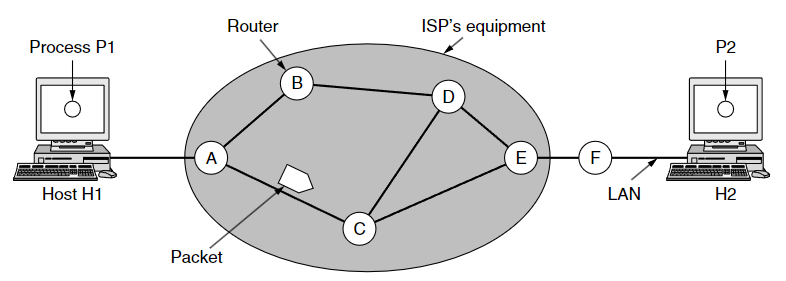
\includegraphics[width=0.309\textwidth]{pic/CN5/The environment of the network layer protocols}
    \caption{The environment of the network layer protocols}
\end{figure}

\subsubsection{Services Provided to the Transport Layer}
Design goals:
\begin{itemize}
    \item The services should be independent of the router technology
    \item The transport layer should be shielded from the number, type, and topology of the routers present
    \item The network addresses should use a uniform numbering plan.
\end{itemize}

Two warring factions, Connection-oriented \& Connectionless service. Network layer should provide connection-oriented service or connectionless service.

The packets are frequently called datagrams. 

\paragraph{Implementation of Connectionless Service}Packets are injected into the network individually and routed independently of each other. 

Every router has a forwarding table. Each table entry is a pair consisting of a destination and the outgoing line to use for that destination.

\begin{figure}[!htb]
    \centering
    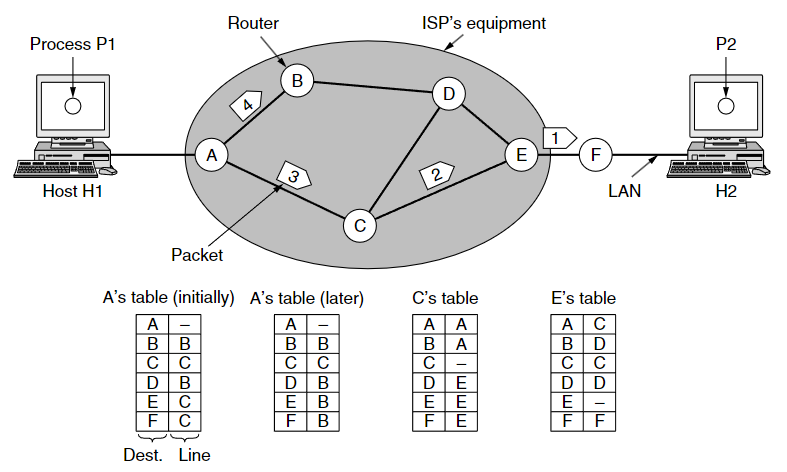
\includegraphics[width=0.309\textwidth]{pic/CN5/Routing within a datagram network}
    \caption{Routing within a datagram network}
\end{figure}


\paragraph{Implementation of Connection-Oriented Service}Each packet carries an identifier telling which virtual circuit it belongs to.

\begin{figure}[!htb]
    \centering
    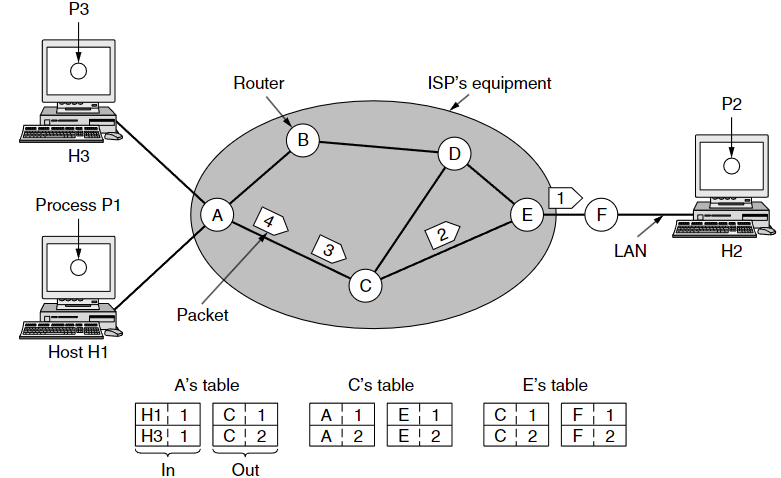
\includegraphics[width=0.309\textwidth]{pic/CN5/Routing within a virtual-circuit network}
    \caption{Routing within a virtual-circuit network}
\end{figure}


\begin{table}[!htb]%TODO P10
    \centering
    \caption{Virtual-Circuit vs. Datagram Networks}
    \begin{tabular}[c]{ccc}\toprule
         \\ \midrule
        
        \bottomrule
    \end{tabular}
\end{table}



\subsection{Routing algorithms}
Two functions of a router: 转发+建立路由表. 

Difference in Datagram and Virtual Circuit:
\begin{itemize}
    \item In datagram, route 实时更新
    \item In virtual circuit, route  仅在初始化时设定
\end{itemize}

\subsubsection{Classification of Routing Algorithms}
Classify routing algorithms into global routing algorithms and decentralized algorithms.
\begin{itemize}
    \item Global routing algorithms: 适用于小网络. e.g. Link-state (LS) algorithms
    \item Decentralized routing algorithms: 适用于大网络. e.g. Distance-vector (DV) algorithms
\end{itemize}

A second broad way to classify routing algorithm:
\begin{itemize}
    \item Static routing algorithms (non-adaptive)
    \item Dynamic routing algorithms (adaptive): 可能会摇摆, 有回路. 
\end{itemize}


\subsubsection{Link-state (LS) algorithms}
In a link-state algorithm, the network topology and all link costs
are known. 首先要 broadcast 以获得这些信息. 

All nodes have an identical and complete view of the network.

The well-known LS algorithm is Dijkstra's algorithm. 

\paragraph{The Shortest Path Algorithm}The shortest path is one that has the least cost. 

Measure path cost (length)
\begin{itemize}
    \item Number of hops
    \item Delay
    \item distance
    \item Bandwidth
    \item Communication cost
    \item Average traffic
\end{itemize}

The optimality principle: If router $J$ is on the optimal path from router $I$ to router $K$, then the optimal path from $J$ to $K$ also falls along the same route.

\paragraph{Sink Tree}
Sink tree for a destination is the union of all shortest paths towards the destination. Similarly source tree. 

Implications:
\begin{enumerate}
    \item Only need to use destination to follow shortest paths
    \item Each node only need to send to the next hop
\end{enumerate}

Forwarding table at a node List next hop for each destination. 

\paragraph{Dijkstra Algorithm}For single source shortest path problem. Approach: Greedy.

The Complexity of Dijkstra Algorithm: worst-case complexity is $O(n^2)$. 

\begin{figure}[!htb]
    \centering
    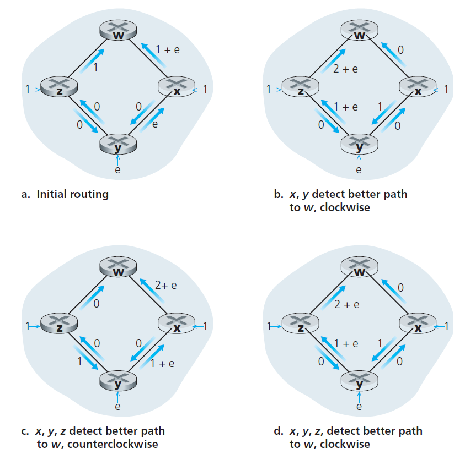
\includegraphics[width=0.309\textwidth]{pic/CN5/Oscillation}
    \caption{The Oscillation Problem with the LS Algorithm}
\end{figure}

\paragraph{Flooding(洪放)}Each router must make decisions based on local knowledge.In flooding, every incoming packet is sent out on every outgoing line except the one it arrived on. 但会有node 接收到重复的拷贝. 

e.g. Consider a flood from A: first reaches B via AB, E via AE. 

\begin{figure}[!htb]
    \centering
    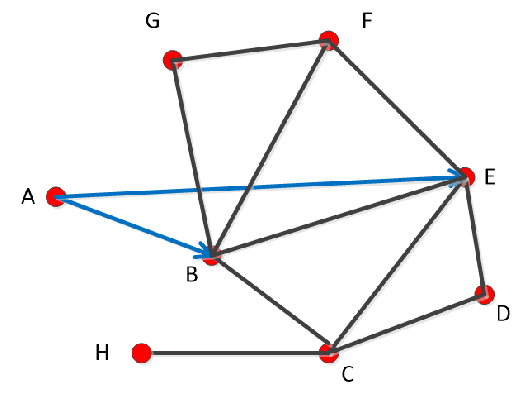
\includegraphics[width=0.309\textwidth]{pic/CN5/Flooding Example}
    \caption{Flooding Example}
\end{figure}

There are some solutions to avoid flooding duplicate packets.
\begin{enumerate}
    \item Solution 1: A hop counter contained in the header of each packet, packet is discarded when the counter reaches zero.
    \item Solution 2: Every node keeps track of which packets have been flooded, to avoid sending them out a second time.
\end{enumerate}

\paragraph{Link State Routing}:
\begin{enumerate}%TODO P45-50
    \item Learning about the neighbors
    \item Setting link costs
    \item Building link state packets
    \subitem The hard part is determining when to build them.
    \item Distributing the link state packets
    \subitem The fundamental idea is to use flooding to distribute the link state packets to all routers.
    \subitem The solution to all these problems is to include the age of each packet
    \subitem To guard against errors on the links, all link state packets are acknowledged.    
    \item Computing the new routes
\end{enumerate}

\subsubsection{Distance-vector (DV) algorithms}
The distance vector routing algorithm is iterative, asynchronous, and distributed. 
\begin{itemize}
    \item Distributed: 从邻居获取信息, 并给邻居信息. 
    \item Iterative: 迭代直到邻居没有信息变更. It is self-terminating. 
    \item Asynchronous: 不要求同步. 
\end{itemize}
DV-like algorithms are used in many routing protocols in practice, including the Internet's RIP, BGP, and so on.

\paragraph{Bellman-Ford Equation}
Let $d_x(y)$ be the cost of the least-cost path from node $x$ to node $y$. Then the least costs are related by the celebrated Bellman-Ford equation, namely,
\begin{align*}
    d_x(y)=\min_v\{ c(x,v)+d_d(y) \}
\end{align*}
where the $\min_v$ in the equation is taken over all of $x$'s neighbors.

\begin{figure}[!htb]
    \centering
    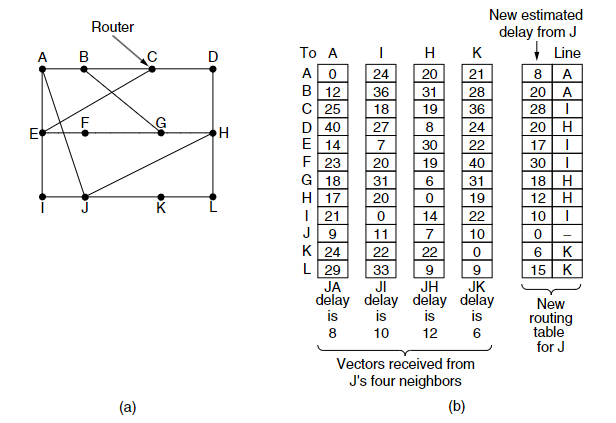
\includegraphics[width=0.309\textwidth]{pic/CN5/Bellman-Ford}
    \caption{(a) A network. (b) Input from $A, I, H, K$, and the new routing table for $J$}
\end{figure}

\paragraph{The Distance Vector Routing Algorithm}
The basic idea: each node $x$ begins with $D_x(y)$, an estimate of the cost of the least-cost path from itself to node $y$, for all nodes in $N$ (the number of nodes in the network). Let $D_x(y) = [D_x(y) : y \in N]$ be node $x$'s distance vector, which is the vector of cost estimates from $x$ to all other nodes, $y \in N$.

With the DV algorithm, each node $x$ maintains the following information:
\begin{itemize}
    \item $c(x, v)$: The cost, for each neighbor node $v$.
    \item $D_x(y)=[D_x(y):y\in N]$: Node $x$'s distance vector.
    \item $D_v(y)=[D_v(y):y\in N]$: The distance vectors of each of its neighbors.
\end{itemize}

\begin{enumerate}
    \item 接受新的 distance vector 后进行更新. 
    \item 有更新就广播给邻居
    \item 直到不变, $D_x(y)$ 收敛于 $d_x(y)$.
\end{enumerate}

最后达到 A quiescent state. 

\paragraph{The Count-to-Infinity Problem}
收敛可能所需时间过长. 

\begin{figure}[!htb]
    \centering
    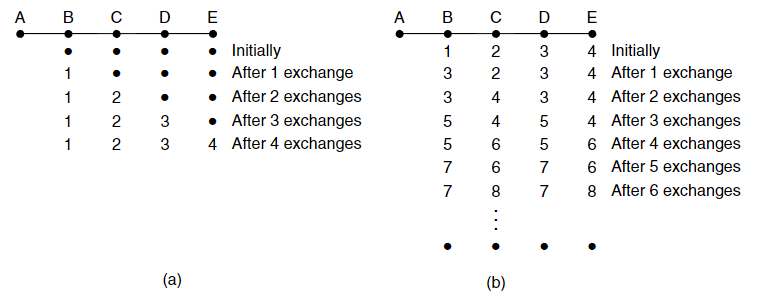
\includegraphics[width=0.42\textwidth]{pic/CN5/The count-to-infinity problem}
    \caption{The count-to-infinity problem}
\end{figure}
Suppose node A is down initially and all other routers know this. In other words, they have all recorded the delay to A as infinity.

\begin{table*}[!htb]
    \centering
    \caption{Distance Vector Routing vs. Link State Routing}
    \begin{tabular}[c]{c|cc}\toprule
        \multicolumn{1}{c}{\textbf{Goal}} & \textbf{Distance Vector} & \textbf{Link State} \\ \midrule
        Correctness & Distributed Bellman-Ford & Replicated Dijkstra's Algorithm \\
        Efficient Paths & Approx. with shortest paths & Approx. with shortest paths \\
        Fair Paths & Approx. with shortest paths & Approx. with shortest paths \\
        Convergence & Slow (many exchanges) & Fast (Flood and compute) \\
        Scalability & Excellent (storage/compute) & Moderate (storage/compute) \\
        \bottomrule
    \end{tabular}
\end{table*}


\subsubsection{Hierarchical Routing}the routers are divided into what we will call regions.

When routing is done hierarchically, there are entries for all the local routers, but all other regions are condensed into a single router.

\subsubsection{Broadcast Routing}the network layer provides a service of delivering a packet sent from a source node to all other nodes in the network. 
\begin{enumerate}
    \item One of the most simple and straightforward way is to send a separate copy of packet to each destination. 
    \item Multidestination routing: Each packet contains either a list of destinations or a bit map indicating the desired destinations
    \item Uncontrolled flooding %TODO 65-68
    \subitem the source node sends a copy of the packet to all of its neighbors
    \subitem Sequence-number-controlled flooding
    \subitem Reverse path forwarding (RPF)
    \item Spanning-Tree Broadcast
    \subitem core: the creation and maintenance of the spanning tree. The center-based approach to building a spanning tree:
    \begin{enumerate}
        \item A center node is defined.
        \item Nodes then unicast tree-join messages addressed to the center
        node. A tree-join message is forwarded using unicast routing
        toward the center until it either arrives at a node that already
        belongs to the spanning tree or arrives at the center.
        \item In either case, the path that the tree-join message has followed
        defines the branch of the spanning tree between the edge node that
        initiated the tree-join message and the center. Graft. 
    \end{enumerate}
\end{enumerate}

\subsubsection{Multicast Routing}%TODO P73-77 自己看

\subsubsection{Anycast Routing}
\begin{itemize}
    \item Unicast --- a single destination
    \item Broadcast --- to all destinations
    \item Multicast --- to a group of destinations
\end{itemize}
In anycast, a packet is delivered to the nearest member of a group. Anycast is used in the Internet as part of DNS. 


\subsection{The network layer in the Internet}
There are two basic choices for connecting different networks:
\begin{enumerate}
    \item build devices that translate or convert packets
    \item building a common layer on top of the different networks.
\end{enumerate}
IP is the foundation of the modern Internet. 

The network layer of the internet has three main components:
\begin{itemize}\small
    \item The IP protocol
    \item The Internet control protocols (including ICMP, DHCP, ARP)
    \item The Internet routing protocols (including RIP, OSPF and BGP)
\end{itemize}

\subsection{IP Protocol}
\subsubsection{The IPv4 Datagram}
The header has a 20-byte fixed part and a variable-length optional part. The bits are transmitted from left to right and top to bottom. This is ``big-endian'' network byte order.

\begin{figure}[!htb]
    \centering
    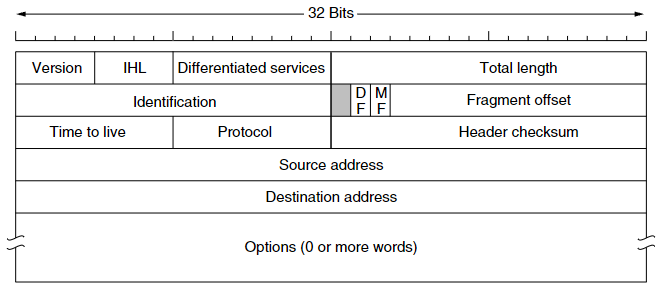
\includegraphics[width=0.42\textwidth]{pic/CN5/The IPv4 (Internet Protocol) header}
    \caption{The IPv4 (Internet Protocol) header}
\end{figure}
\begin{enumerate}
    \item The Version field (4 bits)
    \item IHL field (Header Length) (4 bits)
    \subitem tell how long the header is in 32-bit words, limits the
    header to 60 bytes, thus the options field to 40 bytes. 
    \subitem the typical IP datagram has a 20-bytes header.
    \item The Different Service field (Type of Service) (8 bits)
    \subitem The top 6 bits are used to mark the packet with its service class
    \subitem The bottom 2 bits are used to signal \textbf{explicit congestion indications}
    \item The Total Length field (16 bits)
    \subitem The total length of header and data.
    \subitem The theoretical maximum length is 65,535 bytes.
    \subitem Datagrams are rarely larger than 1,500 bytes. (由 以太网的 MTU 决定)
    \item The Identification field (16 bits), flags (DF, MF), and fragment offset (13 bits)
    \subitem All the fragments of a packet contain the same identification field.
    \begin{itemize}
        \item The Unused bit
        \item DF -- Don't Fragment
        \item MF -- More Fragments 
        \subitem (MF = 0 means this the last fragment)
        \item The Fragment Offset field (13 bits)
        \subitem There is a maximum of 8192 fragments per datagram
    \end{itemize}
    \item The TtL (Time to live) field (8 bit)
    \subitem This field is decremented by one each time the datagram is processed by a router.
    \subitem it just counts hops. When it hits zero, the packet is discarded and a warning packet is sent back to the source host.
    \item The Protocol field (8 bit)
    \subitem tells is which transport process to give the packet to. (6 is TCP, 17 is UDP)
    \subitem The protocol number connect the network and transport layer
    \subitem the port number connect that binds the transport and application layers
    \item The header checksum
    \subitem in the header and using one's complement arithmetic.
    \subitem the checksum must be recomputed and stored again at each router, as the TTL field, and possibly the options fields as well, may change.
    \item The Source address and Destination address (each with 32 bit)
    \item The Options field 用得少
    \item Data (payload)
\end{enumerate}

\paragraph{Packet Fragmentation}
The maximum payloads of different networks
\begin{itemize}
    \item Ethernet -- 1500 bytes
    \item 802.11 -- 2272 bytes
    \item IP -- 65,515 bytes
\end{itemize}

Two Solutions:
\begin{enumerate}
    \item To make sure the packet fragmentation does not occur in the 1st place
    \item To break up packets into fragments, sending each fragment as a separate network layer packet.
\end{enumerate}

Two opposing strategies exist for recombining the fragments back into the original packet
\begin{itemize}
    \item Transparent fragmentation is straightforward but has some problems
    \item Nontransparent fragmentation is to refrain from recombining fragments at any intermediate routers.
\end{itemize}

\begin{figure}[!htb]
    \centering
    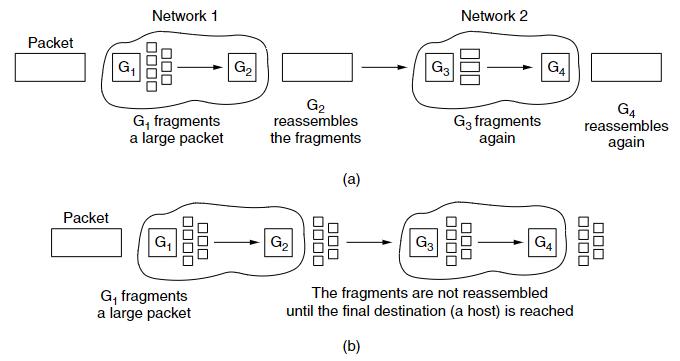
\includegraphics[width=0.42\textwidth]{pic/CN5/recombining the fragments}
    \caption{(a) Transparent fragmentation. (b) Nontransparent fragmentation.}
\end{figure}

e.g. %TODO 94-95

Path MTU discovery

The disadvantage of path MTU discovery is that there may be added startup delays simply to send a packet, more than one round-trip delay may be needed to probe the path

\subsubsection{IPv4 Addressing}
IP 地址有 32 位. 其指向的是一个网络界面, 而不是一台主机. 其是分级的. 其由顶 network portion 与 底 a host portion 组成. IP 也可用 16 进制表示.

% A defining feature of IPv4 is its 32-bit addresses. It is important to note that an IP address does not actually refer to a host. It really refers to a network interface. IP addresses are hierarchical. Each 32-bit address is compromised of a variable-length network portion in the top bits and a host portion in the bottom bits.

Addresses are allocated in blocks called prefixes.
\begin{figure}[!htb]
    \centering
    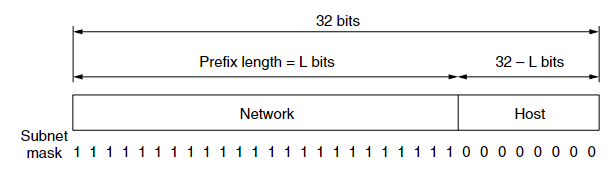
\includegraphics[width=0.42\textwidth]{pic/CN5/An IP prefix and a subnet mask}
    \caption{An IP prefix and a subnet mask}
\end{figure}

\paragraph{IP Prefixes (Network portion)}IP address/length. The /N sometimes known as a subnet mask. 

The key advantage of prefixes is that routers can forward
packets based on only the network portion of the address. 

\paragraph{Subnet}子网个数等于网络中断开路由器后孤岛的个数. 子网 network portion 的地址一致. 将地址块分割成若干部分以供内部用作多个网络. 

\begin{figure}[!htb]
    \centering
    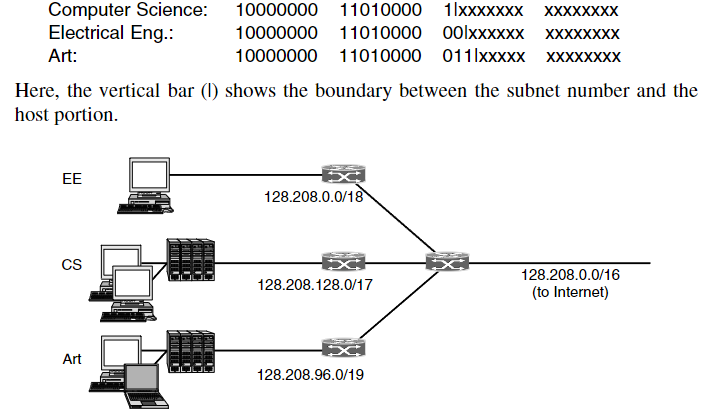
\includegraphics[width=0.42\textwidth]{pic/CN5/Splitting an IP prefix into separate networks with subnetting}
    \caption{Splitting an IP prefix into separate networks with subnetting}
\end{figure}

When a packet comes into the main router, how does the router know which subnet to give it to?
\begin{enumerate}\small
    \item One solution is that for each router to have a table with 65536
    entries telling it which outgoing line to use for each host on
    campus.
    \item The other way is that the router can do this by ANDing the
    destination address with the mask for each subnet and checking
    to see if the result is the corresponding prefix.
\end{enumerate}

\paragraph{IP Address Classes - Historical}Before CIDR, the
network portions of an IP address were constrained to be 8, 16, or 24
bits in length, and addressing scheme known as classful addressing. 

\begin{figure}[!htb]
    \centering
    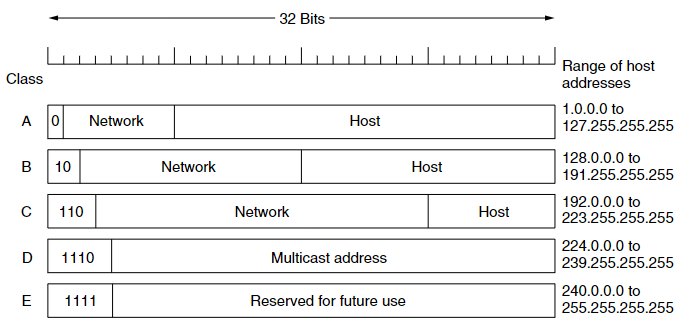
\includegraphics[width=0.42\textwidth]{pic/CN5/IP address formats}
    \caption{IP address formats}
\end{figure}
分配 IP 地址的机构: the Internet
Corporation for Assigned Names and Numbers (ICANN)
following a hierarchical process

\paragraph{Classless InterDomain Routing(CIDR)} There is still a problem: routing table explosion. 

CIDR solution: 
\begin{itemize}
    \item Subnetting: split IP prefixes
    \item Route aggregation: combine multiple small prefixes into
    a single larger prefix.
\end{itemize}

\paragraph{The Longest Matching Prefix}The rule is that packets are sent in the direction of the most
specific route or the longest matching prefix that has the
fewest IP address

% e.g. 172.16.0.0 ABCD 2000, 4000, 4000, 8000
% 172.16.0.0  | 172.16.7.255  | 172.16.0.0/21
% 172.16.16.0 | 172.16.31.255 | 172.16.16.0/20
% 172.16.32.0 | 172.16.47.255 | 172.16.32.0/20
% 172.16.64.0 | 172.16.95.255 | 172.16.64.0/19

\paragraph{Special IP Addresses}\quad 
\begin{itemize}
    \item 0.0.0.0:  means ``this network'' or ``this host''.
    \item 255.255.255.255: mean all hosts on the indicated network, allows broadcasting
    \item 127.0.0.1 (本机地址)
\end{itemize}

\subsubsection{Protocol} %TODO ???

\paragraph{Network Address Translation(NAT)}
IP addresses are scarce.

Solution:
\begin{enumerate}
    \item DHCP
    \item NAT box (Network Address Translation box)
\end{enumerate}

\begin{figure}[!htb]
    \centering
    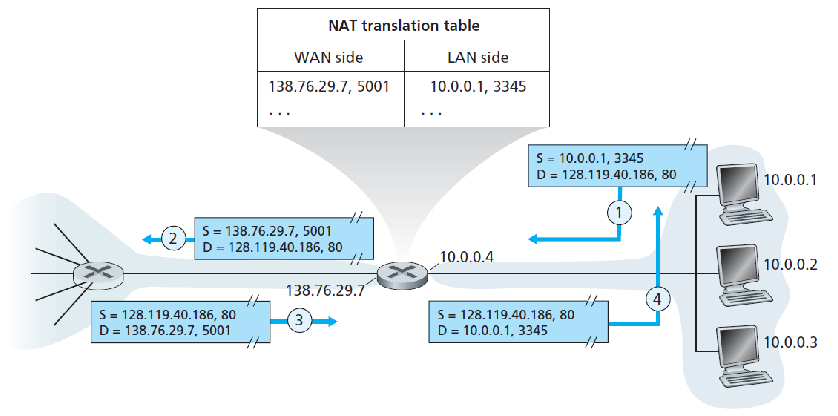
\includegraphics[width=0.42\textwidth]{pic/CN5/Network Address Translation}
    \caption{Network Address Translation}
\end{figure}
The NAT translation table includes port numbers as well as IP addresses in the table entries. 通过端口号区分内部的电脑. 

Ports are effectively an extra 16 bits of addressing that identify which process gets which incoming packet. Ports 0-1023 are reserved for well-known services

Problems with NAT:
\begin{itemize}
    \item Port numbers are meant to be used for addressing processes. 
    \item changes the Internet from a connectionless network to a
    peculiar kind of connection-oriented network.
    \item Routers are supposed to process packets only up to layer 3.
    \item violates the most fundamental rule of protocol layering
\end{itemize}

\paragraph{Dynamic Host Configuration Protocol}DHCP is often referred to as a plug-and-play protocol. DHCP is a client-server protocol, each subnet will have a DHCP server. 

In addition to host IP address assignment, DHCP also allows a host
to learn additional information, such as its subnet mask, the
address of its first-hop router (often called the default gateway),
and the address of its local DNS server.

the DHCP protocol is a four-step process:
\begin{enumerate}\small
    \item DHCP server discovery
    \subitem using a DHCP discover message, which a client
    sends within a UDP packet to port 67.
    \subitem broadcast destination IP address of 255.255.255.255 and a “this
    host” source IP address of 0.0.0.0.
    \item DHCP server offer(s)
    \subitem A DHCP server receiving a DHCP discovery message responds to
    the client with a DHCP offer message that is broadcast to all
    nodes on the subnet
    \subitem Several DHCP servers can be present on the subnet, the client may
    choose from among several offers.
    \item DHCP request
    \subitem The newly arriving client will choose from among one or more
    server offers and respond to its selected offer with a DHCP
    request message echoing back the configuration parameters.
    \item DHCP ACK
    \subitem The server responds to the DHCP request message with a DHCP
    ACK message, confirming the requested parameters.
\end{enumerate}
Once the client receives the DHCP ACK, the interaction is
complete and the client can use the DHCP-allocated IP
address for the lease duration. 

\begin{figure}[!htb]
    \centering
    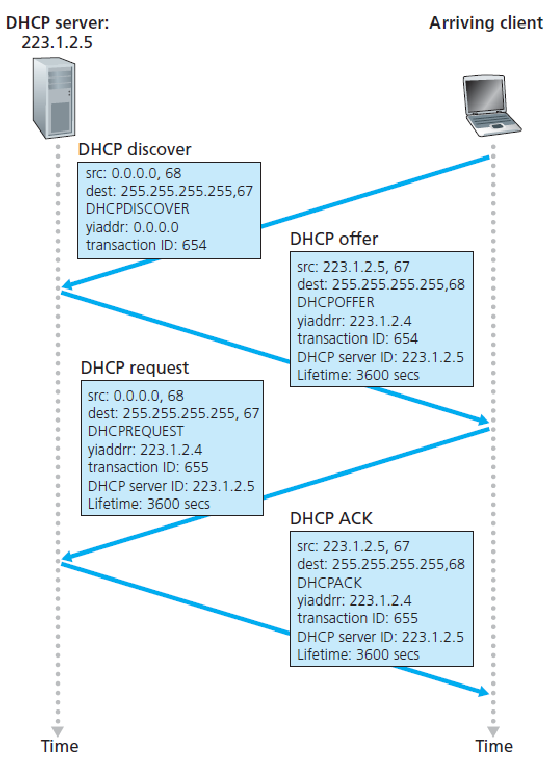
\includegraphics[width=0.309\textwidth]{pic/CN5/DHCP.png}
    \caption{DHCP}
\end{figure}


\subsubsection{IPv6 datagram}
IPv6 uses 128-bit addresses
\begin{figure}[!htb]
    \centering
    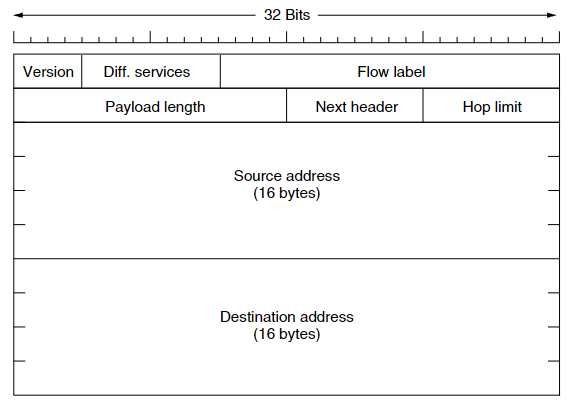
\includegraphics[width=0.42\textwidth]{pic/CN5/The IPv6 fixed header }
    \caption{The IPv6 fixed header }
\end{figure}

\begin{enumerate}%TODO 123-124
    \item the Version field (4 bits)
    \item the Difference Services field (8 bits)
    \item the Flow Label field (20 bits)
    \item the Payload length field (16 bits)
    \item the Next Header field (8 bits)
    \item the Hop Limit field (8 bits)
    \item the Source address and Destination address fields (each
    with 128 bits or 16 bytes)
\end{enumerate}

\subsubsection{The IPv6 Address}
Since many addresses will have many zeros inside them,
three optimization have been authorized:
\begin{enumerate}%TODO 125
    \item 
\end{enumerate}

Several Fields in IPv4 are no longer present in the IPv6 datagram
\begin{itemize}
    \item Fragmentation/reassembly
    \item Header checksum
    \item Options
\end{itemize}

Transitioning from IPv4 to IPv6: two approaches
\begin{enumerate}
    \item IPv6-capable nodes is a dual-stack approach, where IPv6
    nodes also have a complete IPv4 implementation
    \item Tunneling. To take the entire IPv6 datagram into the data
    (payload) field of an IPv4 datagram.
\end{enumerate}

Tunneling %TODO 132


\subsection{Control Protocols}

\subsubsection{Internet Control Message Protocol (ICMP)}
The most typical use of ICMP is for error reporting. ICMP is often considered part of IP but architecturally it lies
just above IP, as ICMP messages are carried inside IP
datagrams.

%TODO P138, note 3 3

\paragraph{Use of ICMP --- ``ping''}\quad

\begin{itemize}
    \item ping sends an ICMP
    type 8 code 0 message (echo request) to the
    specified host.
    \item The destination host, seeing the echo request, sends
    back a type 0 code 0 ICMP echo reply.
\end{itemize}

\paragraph{Use of ICMP --- ``Tracert''}Tracert is implemented with ICMP messages,  to determine
the names and addresses of the routers between source and
destination
\begin{enumerate}\small %TODO 142-144
    \item Tracert in the source sends a series of ordinary IP datagrams to
    the destination.
    \item When the nth datagram arrives at the nth router, the nth router
    observes that the TTL of the datagram has just expired.
    \item When this ICMP message arrives back at the source, the source
    obtains the round-trip time from the timer and the name and IP
    address of the nth router from the ICMP message
    \item How does a Tracert source know when to stop sending UDP segments?
\end{enumerate}

\subsubsection{ARP (The Address Resolution Protocol)}
The purpose of the ARP query packet is to query all the other
nodes on the subnet to determine the MAC address corresponding
to the IP address that is being resolved. 

e.g. How a user on host 1 sends a packet to a user on host 2 on
the CS network? %TODO 152-154
\begin{enumerate}
    \item 
\end{enumerate}

\paragraph{Various Optimizations of ARP}\quad %TODO 156-162
\begin{enumerate}
    \item Cache
    \item The default gateway
    \subitem Through the Default Gateway
    \begin{enumerate}
        \item 
    \end{enumerate}
    \item Proxy ARP
\end{enumerate}

\paragraph{ARP vs. DNS}\quad
\begin{itemize}
    \item ARP resolves an IP address to a MAC address only for nodes on
    the same subnet
    \item DNS resolves host names to IP addresses for hosts anywhere in the
    Internet.
\end{itemize}
ARP is probably best considered a protocol that straddles the boundary between the link and network layers

\subsection{Routing Protocols}
A two-level routing algorithm:
\begin{itemize}
    \item Distance vector routing
    \item Link state routing
\end{itemize}
The networks may all use different intradomain protocols, but they must use the same interdomain protocol. 

\subsubsection{The Internet}
In the network layer, the Internet can be viewed as a collection of networks or ASes (Autonomous Systems) that are interconnected. The glue that holds the whole Internet together is the network layer
protocol, IP (Internet Protocol).

\subsubsection{Autonomous System(AS)}
we will examine two intra-AS routing
protocols (RIP and OSPF) and the inter-AS routing
protocol (BGP) that are used in today's Internet

\paragraph{Intra-AS Routing in the Internet: RIP}RIP (Routing Information Protocol) is a distance-vector protocol. 

RIP uses hop count as a cost metric. %TODO 172
\begin{itemize}
    \item 
\end{itemize}

\begin{enumerate}\small
    \item RIP从已配置接口发送整个路由表,该表以广播或组播(Multicast, 目的地址224.0.0.9)的形式周期性向所有节点发送。
    \item “路由更新”定时器规定了周期性广播或组播的频率,缺省值定为30秒。
    \item 如果达到无效(invalid)超时时间(缺省为180秒)时,路由器仍未收到某路由器的路由更新信息,将把该条路由标记为无效,认为不可达,标记为无效的方式就是将跳数设定为16。
    \item 被标记为不可达的路由仍将保存在路由表里,直到清除定时器超时后,才被清除掉,清除定时器的缺省值为240秒。
    \item 当某一路由项RI包含的目的网络变成不可达到后,该路由项对应的抑制定时器开始计时,在此定时器超时前,即使路由器收到的路由更新指明路由项RI又可达到了,路由项RI仍被本路由器标识为不可到达,只有在抑制定时器超时后,指明路由项RI可到达的路由更新才起作用。抑制定时器的目的在于使路由稳定,不要发生路径摇摆。
\end{enumerate}

\paragraph{OSPF: An Interior Gateway Routing Protocol}% 在实验lab5中讲, 记得搬过来. 
OSPF (Open Shortest Path First,开放式最短路径优先协议). Link state routing. 

The higher data rate, the lower cost of the channel.

\begin{figure}[!htb]
    \centering
    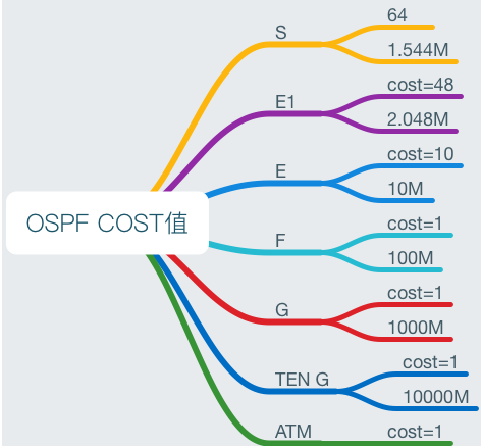
\includegraphics[width=0.309\textwidth]{pic/CN5/OSPF Cost Table}
    \caption{OSPF Cost Table}
\end{figure}

%TODO lab5 15-27, 38

OSPF allows an AS to be divided into numbered areas. An area is a generalization of an individual network. Routers that lie wholly within an area are called internal routers.

Every AS has a backbone area, called area 0. The routers in this area are called backbone routers. All areas are connected to the backbone, possibly by tunnels. 

Each router that is connected to two or more areas is called an area border router (ABR). It must also be part of the backbone. The job of an area border router is to summarize the destinations in one area and to inject this summary into the other areas to which it is connected. This summary includes cost information but not all the details of the topology within an area. If there is only one border router out of an area, even the summary does not need to be passed. This kind of area is called a stub area.

Each router within an area has the same link state database and runs the same shortest path algorithm.

the designed router and A backup designed router

\subsection{BGP: The Exterior Gateway Routing Protocol}
BGP is an absolutely critical protocol for the Internet --- in essence, it is the protocol that glues the whole thing together.

In BGP, pairs of routers exchange routing information over semipermanent TCP connections using port 179. In BGP, destinations are not hosts but instead are CIDRized prefixes. In BGP, an autonomous system is identified by its globally unique autonomous system number (ASN). In BGP jargon, \textit{a prefix along with its attributes} is called \textbf{a route}. %TODO P185 ebgp and ibgp 

\subsubsection{BGP Route Advertising}
Route advertisements contain \textbf{an IP prefix, AS-path, next hop}. Route advertisements move in the opposite direction to traffic.

\begin{figure}[!htb]
    \centering
    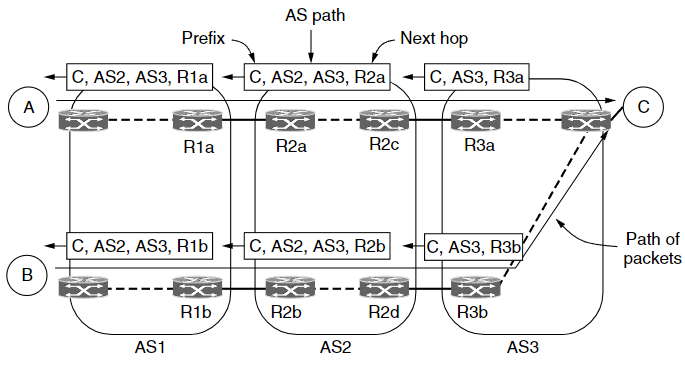
\includegraphics[width=0.42\textwidth]{pic/CN5/Propagation of BGP route advertisements}
    \caption{Propagation of BGP route advertisements}
\end{figure}

TRANSIT service(TR) and PEER service(PE). Note that peering is not transit 

\begin{figure}[!htb]
    \centering
    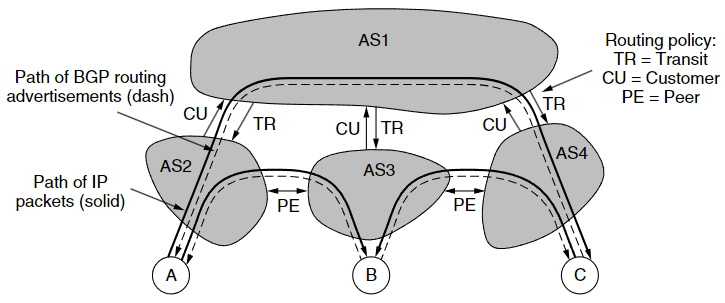
\includegraphics[width=0.42\textwidth]{pic/CN5/Routing policies between four autonomous systems}
    \caption{Routing policies between four autonomous systems}
\end{figure}

\subsubsection{BGP Policy}
Policy is implemented in two ways:
\begin{enumerate}
    \item Border routers of ISP announce paths only to other
    parties who may use those paths
    \item Border routers of ISP select the best path of the ones they
    hear in any, non-shortest way
\end{enumerate}

\subsection{MPLS}
MPLS (Multiprotocol Label Switching) is perilously close to circuit switching. 
\begin{itemize}
    \item To improve the forwarding speed of IP routers by adopting a key
    concept from the world of virtual-circuit networks: a fixed-length
    label
    \item allowing routers to forward datagrams based on fixed-length
    labels (rather than destination IP addresses)
\end{itemize}

\begin{enumerate}
    \item The 1st question to ask is where does the label go?
    \subitem MPLS falls between the network layer protocol and the data link layer protocol. MPLS is sometimes described as a layer 2.5 protocol. 
    \item the 2nd question is to ask when and how the labels are attached to packets?%TODO 196-198
    \subitem Within the MPLS network, the label is used to forward the packet.
    \begin{figure}[!htb]
        \centering
        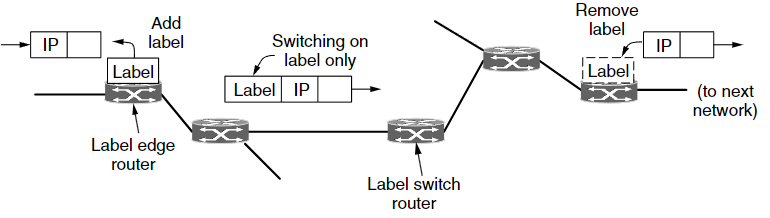
\includegraphics[width=0.42\textwidth]{pic/CN5/Forwarding an IP packet through an MPLS network}
        \caption{Forwarding an IP packet through an MPLS network}
    \end{figure}
    \item The final question we will ask is how the label forwarding tables are set up so that packets follow them %TODO P199-200
    \subitem a setup packet is launched into the
    network to create the path and make the forwarding table entries. allocates a label for each
    one and passes the labels to its neighbors. 
\end{enumerate}

\subsection{Internet Multicasting}
IP supports one-to-many communication, or multicasting, using class D IP addresses. 28 bits are available for identifying groups, so over 250 million
groups can exist at the same time.

Some examples of local multicast addresses are:
\begin{itemize}%TODO 201
    \item 
\end{itemize}

